\documentclass{article}
\usepackage[letterpaper, portrait, margin=1in]{geometry}
\usepackage[capitalise]{cleveref}
\usepackage{import}
\usepackage{booktabs}
\usepackage{multirow}
\usepackage{csvsimple}
\usepackage{longtable}
\usepackage{graphicx}
\usepackage{listings}
\usepackage{minted}
\usepackage{caption}
\usepackage{pdflscape}

\newcommand\ddg{$\Delta\Delta G$}

\usepackage{xr} % Probably not needed for submission
\externaldocument{flex-ddG}

% A listing of the contents of each file supplied as Supporting Information
% should be included. For instructions on what should be included in the
% Supporting Information as well as how to prepare this material for
% publications, refer to the journal's Instructions for Authors.

% The following files are available free of charge.
% \begin{itemize}
% \item Filename: brief description
% \item Filename: brief description
% \end{itemize}

% Supplementary figures:
% \begin{itemize}
% \item \cref{tab:table-mult}
% \item \cref{fig:steps-v-corr}
% \item \cref{tab:table-versions}
% \item \cref{fig:structs-v-corr-id-zemu-12-60000-rscript-validated-t14}
% \item \cref{fig:structs-v-corr-WildTypeComplex-ddg-monomer-16-003-zemu-2}
% \item \cref{fig:wildtypecomplex-scores-complete}
% \item \cref{fig:spear-corr-rmsd-error}
% \item \cref{fig:t14-mean-ensemble}
% \item \cref{tab:table-ref}
% \item \cref{tab:table-antibodies}
% \item \cref{fig:t14-fits-feats}
% \end{itemize}

\begin{document}

\renewcommand{\thefigure}{S\arabic{figure}}
\setcounter{figure}{0}
\renewcommand{\thetable}{S\arabic{table}}
\setcounter{table}{0}
% \renewcommand{\lstlistingname}{Supporting Listing}

\subimport*{figs-and-tables/}{table-versions}
\subimport*{figs-and-tables/}{table-temperature}
\subimport*{figs-and-tables/}{table-stabilizing}
\clearpage
{\small
\begin{longtable}{llrrrr}
\toprule
Mutation Category &   Prediction Method &   N &     R &  MAE &   FC \\
\midrule
 \multirow{ 4}{*}{pdb-1A22} & flex ddG & \multirow{ 4}{*}{142} & \textbf{0.32} & \textbf{0.61} & \textbf{0.79}  \\
 & no backrub control & & 0.18 & 0.77 & 0.74  \\
 & ddG monomer & & 0.12 & 0.91 & 0.73  \\
 & ZEMu paper & & 0.19 & 0.68 & 0.78  \\
\hline
 \multirow{ 4}{*}{pdb-1A4Y} & flex ddG & \multirow{ 4}{*}{45} & 0.81 & 1.34 & 0.71  \\
 & no backrub control & & 0.79 & 1.47 & \textbf{0.78}  \\
 & ddG monomer & & 0.77 & 1.91 & 0.62  \\
 & ZEMu paper & & \textbf{0.87} & \textbf{1.12} & 0.73  \\
\hline
 \multirow{ 4}{*}{pdb-1ACB} & flex ddG & \multirow{ 4}{*}{6} & 0.28 & 2.89 & 0.83  \\
 & no backrub control & & 0.23 & 2.37 & 0.83  \\
 & ddG monomer & & 0.58 & \textbf{1.57} & \textbf{1.00}  \\
 & ZEMu paper & & \textbf{0.79} & 2.17 & 0.83  \\
\hline
 \multirow{ 4}{*}{pdb-1AHW} & flex ddG & \multirow{ 4}{*}{10} & -0.83 & 1.31 & 0.4  \\
 & no backrub control & & -0.42 & 1.42 & 0.4  \\
 & ddG monomer & & -0.34 & 1.26 & 0.5  \\
 & ZEMu paper & & \textbf{0.30} & \textbf{0.93} & \textbf{0.6}  \\
\hline
 \multirow{ 4}{*}{pdb-1AK4} & flex ddG & \multirow{ 4}{*}{15} & \textbf{0.73} & \textbf{0.53} & \textbf{0.73}  \\
 & no backrub control & & 0.35 & 1.01 & 0.47  \\
 & ddG monomer & & 0.63 & 1.35 & 0.60  \\
 & ZEMu paper & & 0.44 & 1.63 & 0.53  \\
\hline
 \multirow{ 4}{*}{pdb-1CBW} & flex ddG & \multirow{ 4}{*}{15} & 0.01 & \textbf{0.59} & \textbf{0.87}  \\
 & no backrub control & & \textbf{0.05} & 0.83 & 0.67  \\
 & ddG monomer & & -0.09 & 0.72 & 0.67  \\
 & ZEMu paper & & -0.26 & 0.71 & 0.67  \\
\hline
 \multirow{ 4}{*}{pdb-1CSE} & flex ddG & \multirow{ 4}{*}{6} & 0.44 & 1.94 & 0.67  \\
 & no backrub control & & 0.37 & 2.03 & 0.67  \\
 & ddG monomer & & 0.46 & 1.88 & 0.67  \\
 & ZEMu paper & & \textbf{0.87} & \textbf{0.81} & \textbf{1.00}  \\
\hline
 \multirow{ 4}{*}{pdb-1DAN} & flex ddG & \multirow{ 4}{*}{118} & 0.65 & \textbf{0.53} & \textbf{0.88}  \\
 & no backrub control & & \textbf{0.69} & 0.59 & 0.85  \\
 & ddG monomer & & 0.61 & 0.71 & 0.83  \\
 & ZEMu paper & & 0.32 & 0.88 & 0.76  \\
\hline
 \multirow{ 4}{*}{pdb-1DFJ} & flex ddG & \multirow{ 4}{*}{20} & 0.70 & 1.35 & \textbf{0.70}  \\
 & no backrub control & & \textbf{0.83} & \textbf{1.04} & 0.60  \\
 & ddG monomer & & 0.69 & 1.38 & 0.55  \\
 & ZEMu paper & & 0.55 & 1.40 & 0.55  \\
\hline
 \multirow{ 4}{*}{pdb-1DQJ} & flex ddG & \multirow{ 4}{*}{34} & \textbf{0.44} & \textbf{1.67} & 0.79  \\
 & no backrub control & & 0.39 & 1.93 & 0.65  \\
 & ddG monomer & & 0.37 & 1.87 & \textbf{0.82}  \\
 & ZEMu paper & & 0.28 & 2.08 & 0.59  \\
\hline
 \multirow{ 4}{*}{pdb-1DVF} & flex ddG & \multirow{ 4}{*}{38} & 0.63 & 1.58 & 0.53  \\
 & no backrub control & & \textbf{0.65} & \textbf{1.50} & 0.66  \\
 & ddG monomer & & 0.61 & 1.54 & \textbf{0.71}  \\
 & ZEMu paper & & 0.57 & 1.54 & 0.53  \\
\hline
 \multirow{ 4}{*}{pdb-1E96} & flex ddG & \multirow{ 4}{*}{6} & \textbf{0.52} & \textbf{0.84} & 0.50  \\
 & no backrub control & & 0.51 & 0.91 & 0.50  \\
 & ddG monomer & & 0.45 & 0.96 & 0.50  \\
 & ZEMu paper & & 0.50 & 0.85 & \textbf{0.67}  \\
\hline
 \multirow{ 4}{*}{pdb-1EAW} & flex ddG & \multirow{ 4}{*}{27} & 0.03 & 0.58 & 0.85  \\
 & no backrub control & & 0.07 & 0.73 & 0.81  \\
 & ddG monomer & & \textbf{0.13} & 0.61 & 0.89  \\
 & ZEMu paper & & 0.00 & \textbf{0.49} & \textbf{0.93}  \\
\hline
 \multirow{ 4}{*}{pdb-1EMV} & flex ddG & \multirow{ 4}{*}{51} & \textbf{0.89} & \textbf{0.86} & \textbf{0.86}  \\
 & no backrub control & & 0.84 & 0.98 & 0.84  \\
 & ddG monomer & & 0.84 & 0.96 & 0.80  \\
 & ZEMu paper & & 0.87 & 0.89 & 0.84  \\
\hline
 \multirow{ 4}{*}{pdb-1F47} & flex ddG & \multirow{ 4}{*}{12} & 0.56 & \textbf{0.72} & 0.50  \\
 & no backrub control & & 0.58 & 0.87 & \textbf{0.58}  \\
 & ddG monomer & & \textbf{0.60} & 0.87 & \textbf{0.58}  \\
 & ZEMu paper & & 0.51 & 1.02 & 0.42  \\
\hline
 \multirow{ 4}{*}{pdb-1FC2} & flex ddG & \multirow{ 4}{*}{9} & -0.07 & \textbf{0.84} & 0.56  \\
 & no backrub control & & -0.09 & 1.01 & 0.67  \\
 & ddG monomer & & -0.39 & 1.19 & 0.44  \\
 & ZEMu paper & & \textbf{0.28} & 0.89 & \textbf{0.78}  \\
\hline
 \multirow{ 4}{*}{pdb-1FCC} & flex ddG & \multirow{ 4}{*}{8} & -0.21 & 1.56 & \textbf{0.5}  \\
 & no backrub control & & -0.22 & 1.96 & \textbf{0.5}  \\
 & ddG monomer & & -0.06 & 1.50 & \textbf{0.5}  \\
 & ZEMu paper & & \textbf{0.16} & \textbf{1.35} & \textbf{0.5}  \\
\hline
 \multirow{ 4}{*}{pdb-1GC1} & flex ddG & \multirow{ 4}{*}{56} & 0.12 & \textbf{0.35} & \textbf{0.91}  \\
 & no backrub control & & -0.15 & 0.43 & 0.86  \\
 & ddG monomer & & 0.28 & 0.38 & 0.86  \\
 & ZEMu paper & & \textbf{0.36} & 0.55 & 0.84  \\
\hline
 \multirow{ 4}{*}{pdb-1HE8} & flex ddG & \multirow{ 4}{*}{10} & 0.39 & 0.67 & \textbf{0.5}  \\
 & no backrub control & & 0.62 & 0.91 & \textbf{0.5}  \\
 & ddG monomer & & 0.26 & \textbf{0.66} & 0.3  \\
 & ZEMu paper & & \textbf{0.81} & 1.23 & \textbf{0.5}  \\
\hline
 \multirow{ 4}{*}{pdb-1IAR} & flex ddG & \multirow{ 4}{*}{36} & 0.64 & \textbf{0.72} & 0.78  \\
 & no backrub control & & 0.35 & 1.32 & 0.67  \\
 & ddG monomer & & \textbf{0.66} & 0.98 & \textbf{0.81}  \\
 & ZEMu paper & & 0.45 & 0.86 & 0.78  \\
\hline
 \multirow{ 4}{*}{pdb-1JCK} & flex ddG & \multirow{ 4}{*}{7} & 0.46 & 1.22 & 0.57  \\
 & no backrub control & & 0.44 & 0.97 & \textbf{0.71}  \\
 & ddG monomer & & 0.75 & 1.25 & \textbf{0.71}  \\
 & ZEMu paper & & \textbf{0.85} & \textbf{0.94} & \textbf{0.71}  \\
\hline
 \multirow{ 4}{*}{pdb-1JRH} & flex ddG & \multirow{ 4}{*}{53} & \textbf{0.58} & \textbf{1.09} & 0.66  \\
 & no backrub control & & 0.50 & 1.25 & 0.60  \\
 & ddG monomer & & 0.52 & 1.29 & \textbf{0.75}  \\
 & ZEMu paper & & 0.57 & 1.15 & 0.58  \\
\hline
 \multirow{ 4}{*}{pdb-1JTG} & flex ddG & \multirow{ 4}{*}{118} & 0.44 & 1.87 & 0.84  \\
 & no backrub control & & 0.39 & \textbf{1.77} & 0.83  \\
 & ddG monomer & & 0.40 & 2.12 & \textbf{0.86}  \\
 & ZEMu paper & & \textbf{0.51} & \textbf{1.77} & 0.75  \\
\hline
 \multirow{ 4}{*}{pdb-1KTZ} & flex ddG & \multirow{ 4}{*}{27} & \textbf{0.86} & \textbf{0.63} & 0.74  \\
 & no backrub control & & 0.76 & 1.16 & \textbf{0.85}  \\
 & ddG monomer & & 0.71 & 1.13 & 0.81  \\
 & ZEMu paper & & 0.80 & 0.83 & 0.70  \\
\hline
 \multirow{ 4}{*}{pdb-1LFD} & flex ddG & \multirow{ 4}{*}{25} & \textbf{0.55} & \textbf{0.68} & \textbf{0.72}  \\
 & no backrub control & & 0.13 & 1.21 & 0.60  \\
 & ddG monomer & & 0.28 & 0.97 & \textbf{0.72}  \\
 & ZEMu paper & & 0.27 & 0.84 & 0.60  \\
\hline
 \multirow{ 4}{*}{pdb-1MLC} & flex ddG & \multirow{ 4}{*}{16} & -0.28 & 1.01 & 0.62  \\
 & no backrub control & & 0.22 & 0.82 & 0.75  \\
 & ddG monomer & & 0.28 & 0.83 & 0.56  \\
 & ZEMu paper & & \textbf{0.79} & \textbf{0.42} & \textbf{0.88}  \\
\hline
 \multirow{ 4}{*}{pdb-1NMB} & flex ddG & \multirow{ 4}{*}{6} & 0.21 & 0.83 & \textbf{0.83}  \\
 & no backrub control & & 0.48 & 0.83 & 0.67  \\
 & ddG monomer & & 0.62 & \textbf{0.60} & \textbf{0.83}  \\
 & ZEMu paper & & \textbf{0.78} & 1.97 & 0.17  \\
\hline
 \multirow{ 4}{*}{pdb-1REW} & flex ddG & \multirow{ 4}{*}{24} & \textbf{0.89} & \textbf{0.67} & \textbf{0.92}  \\
 & no backrub control & & 0.78 & 1.19 & 0.75  \\
 & ddG monomer & & 0.76 & 1.20 & 0.79  \\
 & ZEMu paper & & 0.65 & 1.03 & \textbf{0.92}  \\
\hline
 \multirow{ 4}{*}{pdb-1S1Q} & flex ddG & \multirow{ 4}{*}{6} & 0.17 & \textbf{0.68} & \textbf{0.67}  \\
 & no backrub control & & 0.22 & 0.75 & \textbf{0.67}  \\
 & ddG monomer & & \textbf{0.34} & 0.71 & \textbf{0.67}  \\
 & ZEMu paper & & -0.07 & 1.09 & 0.50  \\
\hline
 \multirow{ 4}{*}{pdb-1TM1} & flex ddG & \multirow{ 4}{*}{21} & 0.33 & 1.71 & 0.43  \\
 & no backrub control & & 0.23 & 1.81 & 0.43  \\
 & ddG monomer & & 0.23 & 1.72 & 0.62  \\
 & ZEMu paper & & \textbf{0.58} & \textbf{1.37} & \textbf{0.71}  \\
\hline
 \multirow{ 4}{*}{pdb-1UUZ} & flex ddG & \multirow{ 4}{*}{5} & 0.79 & 0.62 & \textbf{0.8}  \\
 & no backrub control & & \textbf{0.92} & \textbf{0.52} & \textbf{0.8}  \\
 & ddG monomer & & 0.83 & 0.80 & \textbf{0.8}  \\
 & ZEMu paper & & 0.42 & 1.60 & 0.2  \\
\hline
 \multirow{ 4}{*}{pdb-1VFB} & flex ddG & \multirow{ 4}{*}{43} & 0.58 & \textbf{0.95} & \textbf{0.70}  \\
 & no backrub control & & 0.21 & 1.50 & 0.67  \\
 & ddG monomer & & \textbf{0.64} & 1.40 & \textbf{0.70}  \\
 & ZEMu paper & & 0.60 & 1.07 & 0.65  \\
\hline
 \multirow{ 4}{*}{pdb-1XD3} & flex ddG & \multirow{ 4}{*}{18} & 0.46 & 0.95 & 0.72  \\
 & no backrub control & & 0.28 & 1.43 & 0.67  \\
 & ddG monomer & & 0.51 & 1.15 & 0.67  \\
 & ZEMu paper & & \textbf{0.56} & \textbf{0.71} & \textbf{0.83}  \\
\hline
 \multirow{ 4}{*}{pdb-2I9B} & flex ddG & \multirow{ 4}{*}{5} & -0.81 & 0.53 & \textbf{1.0}  \\
 & no backrub control & & -0.00 & \textbf{0.49} & \textbf{1.0}  \\
 & ddG monomer & & -0.56 & 0.55 & \textbf{1.0}  \\
 & ZEMu paper & & \textbf{0.65} & 0.62 & \textbf{1.0}  \\
\hline
 \multirow{ 4}{*}{pdb-2JEL} & flex ddG & \multirow{ 4}{*}{43} & \textbf{0.67} & 0.64 & \textbf{0.84}  \\
 & no backrub control & & 0.62 & \textbf{0.63} & 0.81  \\
 & ddG monomer & & 0.64 & 0.70 & \textbf{0.84}  \\
 & ZEMu paper & & 0.48 & 0.81 & 0.74  \\
\hline
 \multirow{ 4}{*}{pdb-2PCB} & flex ddG & \multirow{ 4}{*}{6} & \textbf{0.28} & \textbf{0.44} & \textbf{1.00}  \\
 & no backrub control & & 0.23 & 0.64 & 0.67  \\
 & ddG monomer & & -0.70 & 0.90 & \textbf{1.00}  \\
 & ZEMu paper & & -0.63 & 0.95 & 0.83  \\
\hline
 \multirow{ 4}{*}{pdb-2PCC} & flex ddG & \multirow{ 4}{*}{12} & \textbf{0.10} & \textbf{1.27} & \textbf{0.5}  \\
 & no backrub control & & 0.04 & 1.49 & \textbf{0.5}  \\
 & ddG monomer & & -0.29 & 1.90 & \textbf{0.5}  \\
 & ZEMu paper & & -0.24 & 1.53 & \textbf{0.5}  \\
\hline
 \multirow{ 4}{*}{pdb-2VLJ} & flex ddG & \multirow{ 4}{*}{14} & 0.40 & \textbf{0.84} & 0.57  \\
 & no backrub control & & \textbf{0.42} & 1.75 & 0.43  \\
 & ddG monomer & & 0.26 & 0.93 & 0.50  \\
 & ZEMu paper & & 0.15 & 0.89 & \textbf{0.64}  \\
\hline
 \multirow{ 4}{*}{pdb-2WPT} & flex ddG & \multirow{ 4}{*}{32} & 0.54 & 1.60 & 0.62  \\
 & no backrub control & & \textbf{0.63} & \textbf{1.39} & \textbf{0.75}  \\
 & ddG monomer & & 0.56 & 1.63 & 0.69  \\
 & ZEMu paper & & 0.45 & 1.63 & 0.56  \\
\hline
 \multirow{ 4}{*}{pdb-3BK3} & flex ddG & \multirow{ 4}{*}{13} & \textbf{0.72} & \textbf{0.51} & 0.69  \\
 & no backrub control & & 0.70 & 0.98 & 0.62  \\
 & ddG monomer & & 0.65 & 0.55 & \textbf{0.85}  \\
 & ZEMu paper & & 0.31 & 1.45 & 0.54  \\
\hline
 \multirow{ 4}{*}{pdb-3BN9} & flex ddG & \multirow{ 4}{*}{25} & 0.48 & \textbf{0.39} & \textbf{0.88}  \\
 & no backrub control & & \textbf{0.53} & 0.40 & \textbf{0.88}  \\
 & ddG monomer & & 0.31 & 0.66 & \textbf{0.88}  \\
 & ZEMu paper & & -0.09 & 0.66 & 0.84  \\
\hline
 \multirow{ 4}{*}{pdb-3NPS} & flex ddG & \multirow{ 4}{*}{27} & 0.18 & \textbf{0.71} & 0.74  \\
 & no backrub control & & \textbf{0.26} & 0.87 & \textbf{0.78}  \\
 & ddG monomer & & 0.15 & 0.84 & \textbf{0.78}  \\
 & ZEMu paper & & -0.21 & 0.89 & 0.67  \\
\bottomrule
  \caption[Flex ddG performance by PDB structure for all complexes with 5 or more cases]{
    Flex ddG performance by PDB structure for all complexes with 5 or more cases. Backrub steps = 35000. N = number of cases (variants) for each complex. R = Pearson's R. MAE = Mean Absolute Error. FC = Fraction Correct. Best performance for each metric and dataset is shown in bold.
  } \label{tab:table-by-structure}
\end{longtable}

}
\clearpage

\begin{landscape}
\subimport*{figs-and-tables/}{structs-v-corr-WildTypeComplex-zemu-12-60000-rscript-validated-t14-underlying-data}
\end{landscape}
\clearpage

\begin{figure}
  \centering
  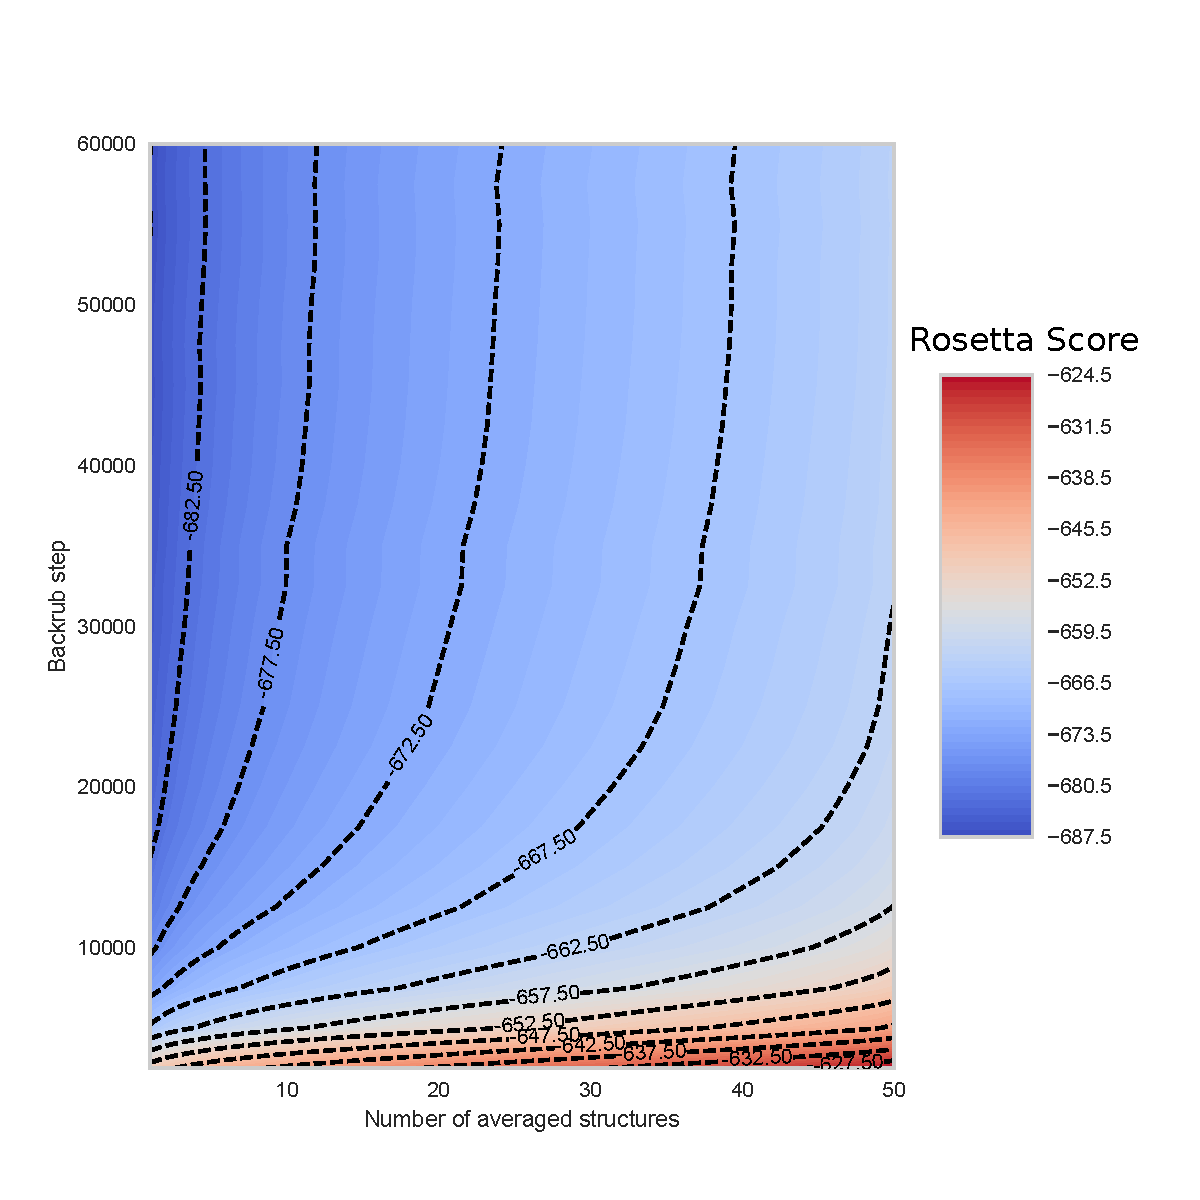
\includegraphics[width=\textwidth,keepaspectratio]{figures/wildtypecomplex-scores-complete.pdf}
  \caption{
    Contour plot showing the effect of backrub sampling on the average wild-type complex score, for increasing numbers of averaged models. As the number of averaged structures N$_{struct}$ is increased along the x-axis, the average total score of the ensemble of modeled wild-type complexes (shown as colored contours in the body of the plot) also increases, as the wild-type complex models are first sorted according to their total scores and included in the averaged ensemble in order of increasing score.
    As the number of backrub sampling steps at which the ensemble is generated increases (along the y-axis), the total score of an ensemble of any number of structures tends to decrease, indicating that flex ddG is able to find lower-energy states (as measured by the Rosetta energy function) as the simulation progresses. However, using only the lowest energy structures does not produce higher correlations with experimental \ddg\ values, as shown in \cref{fig:structs-v-corr-WildTypeComplex-zemu-12-60000-rscript-validated-t14}.
  } \label{fig:wildtypecomplex-scores-complete}
\end{figure}

\subimport*{figs-and-tables/}{structs-v-corr-WildTypeComplex-ddg-monomer-16-003-zemu-2}
\clearpage
\begin{landscape}
\subimport*{figs-and-tables/}{structs-v-corr-WildTypeComplex-ddg-monomer-16-003-zemu-2-underlying-data}
\end{landscape}
\clearpage

\subimport*{figs-and-tables/}{structs-v-corr-id-zemu-12-60000-rscript-validated-t14}
\clearpage
\begin{landscape}
\subimport*{figs-and-tables/}{structs-v-corr-id-zemu-12-60000-rscript-validated-t14-underlying-data}
\end{landscape}
\clearpage

\begin{figure}
  \centering
  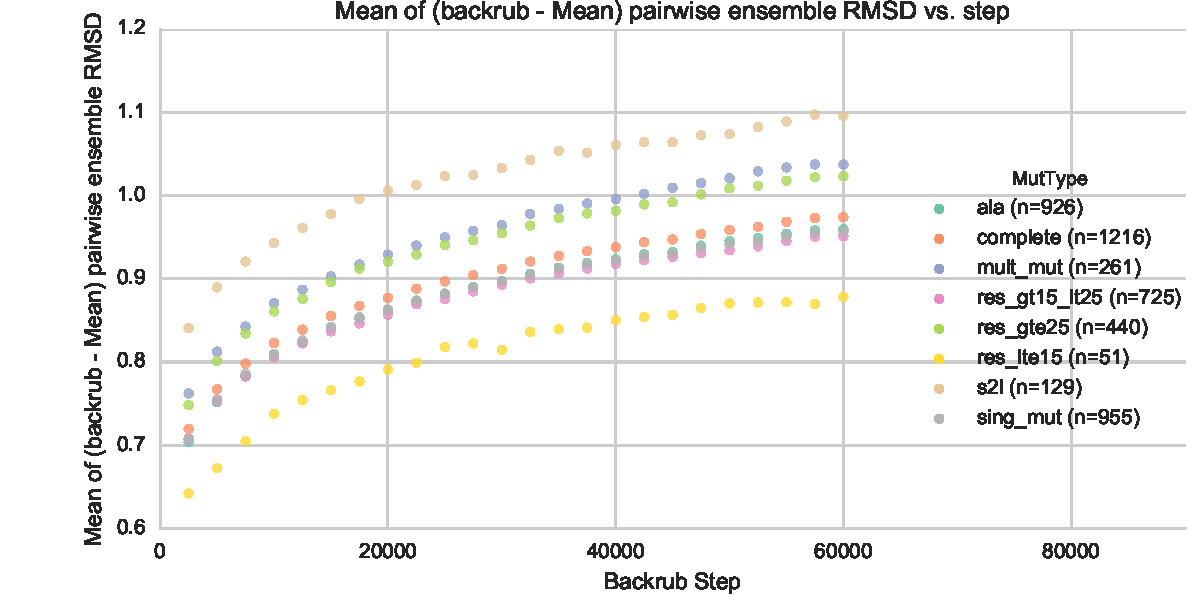
\includegraphics[width=\textwidth,keepaspectratio]{figures/t14-mean-ensemble-error.pdf}
  \caption{
    The average pairwise ensemble RMSD for each ensemble of 50 structures is shown versus increasing backrub sampling steps. Average pairwise RMSD is computed on the mean of all atoms in all residues selected as backrub pivots, superimposed onto the last output structure in the trajectory. For all analyzed subsets, including the complete dataset, pairwise ensemble RMSD increases with increasing backrub sampling steps, indicating that the diversity of sampled models (as measured by RMSD) continues to increase past the point around 30k-35k sampling steps where correlation with experimental \ddg\ values levels out. Subset legend: ala = mutation(s) to alanine; complete = complete ZEMu dataset; mult\_mut = multiple mutations (per data point); res\_gt15\_lt25 = resolution of the input wild-type structure $> 1.5\ \AA$ and $< 2.5\ \AA$; res\_gte25 = resolution of the input wild-type structure $>=\ 2.5\ \AA$; res\_lte15 = resolution of the input wild-type structure $<=\ 1.5\ \AA$; s2l = small-to-large mutation(s); sing\_mut = single mutations. N = number of cases in each subset.
  } \label{fig:t14-mean-ensemble}
\end{figure}

% \begin{figure}
%   \centering
%   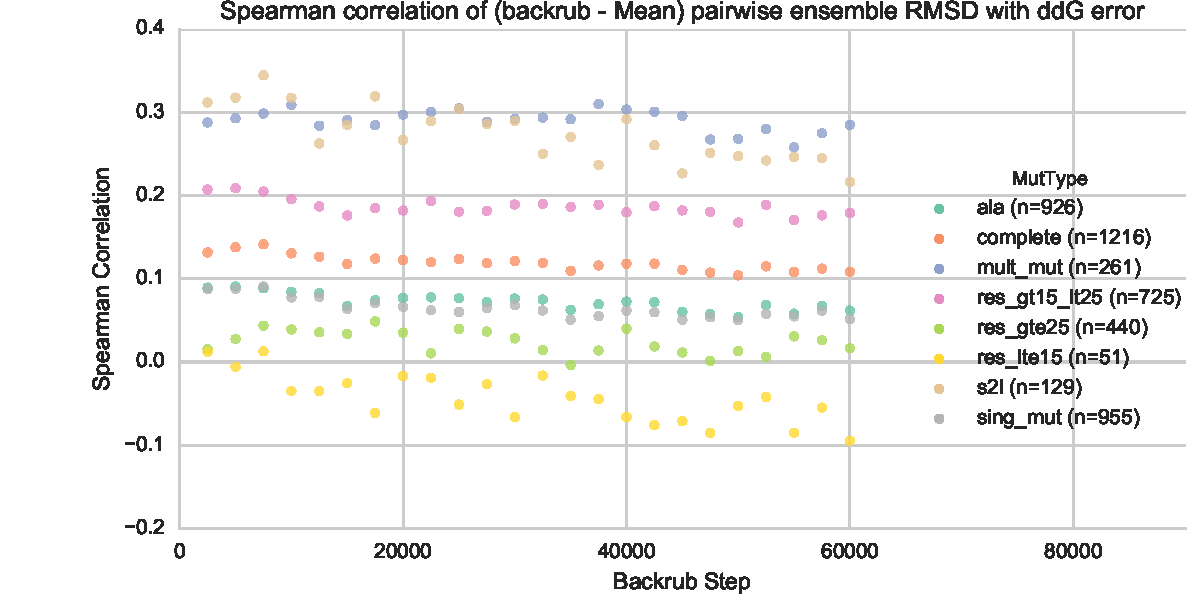
\includegraphics[width=\textwidth,keepaspectratio]{figures/t14-spear-corr.pdf}
%   \caption[\ddg\ prediction error vs. ensemble RMSD]{
%     Scatter plot showing the average Spearman correlation of ddG prediction error v. mean pairwise backrub ensemble RMSD, v. backrub steps.
%     As mean backrub ensemble RMSD increases (\cref{fig:t14-mean-ensemble}), we do not see any significant change in Spearman rank-order correlation between mean ensemble RMSD and ddG error (y-axis), as backrub steps increase (x-axis).
%     This demonstrates that mean pairwise backrub ensemble RMSD might not be an effective metric to measure the degree to which we have sampled ``enough''.
%   } \label{fig:spear-corr-rmsd-error}
% \end{figure}

% \begin{figure}
%   \centering
%   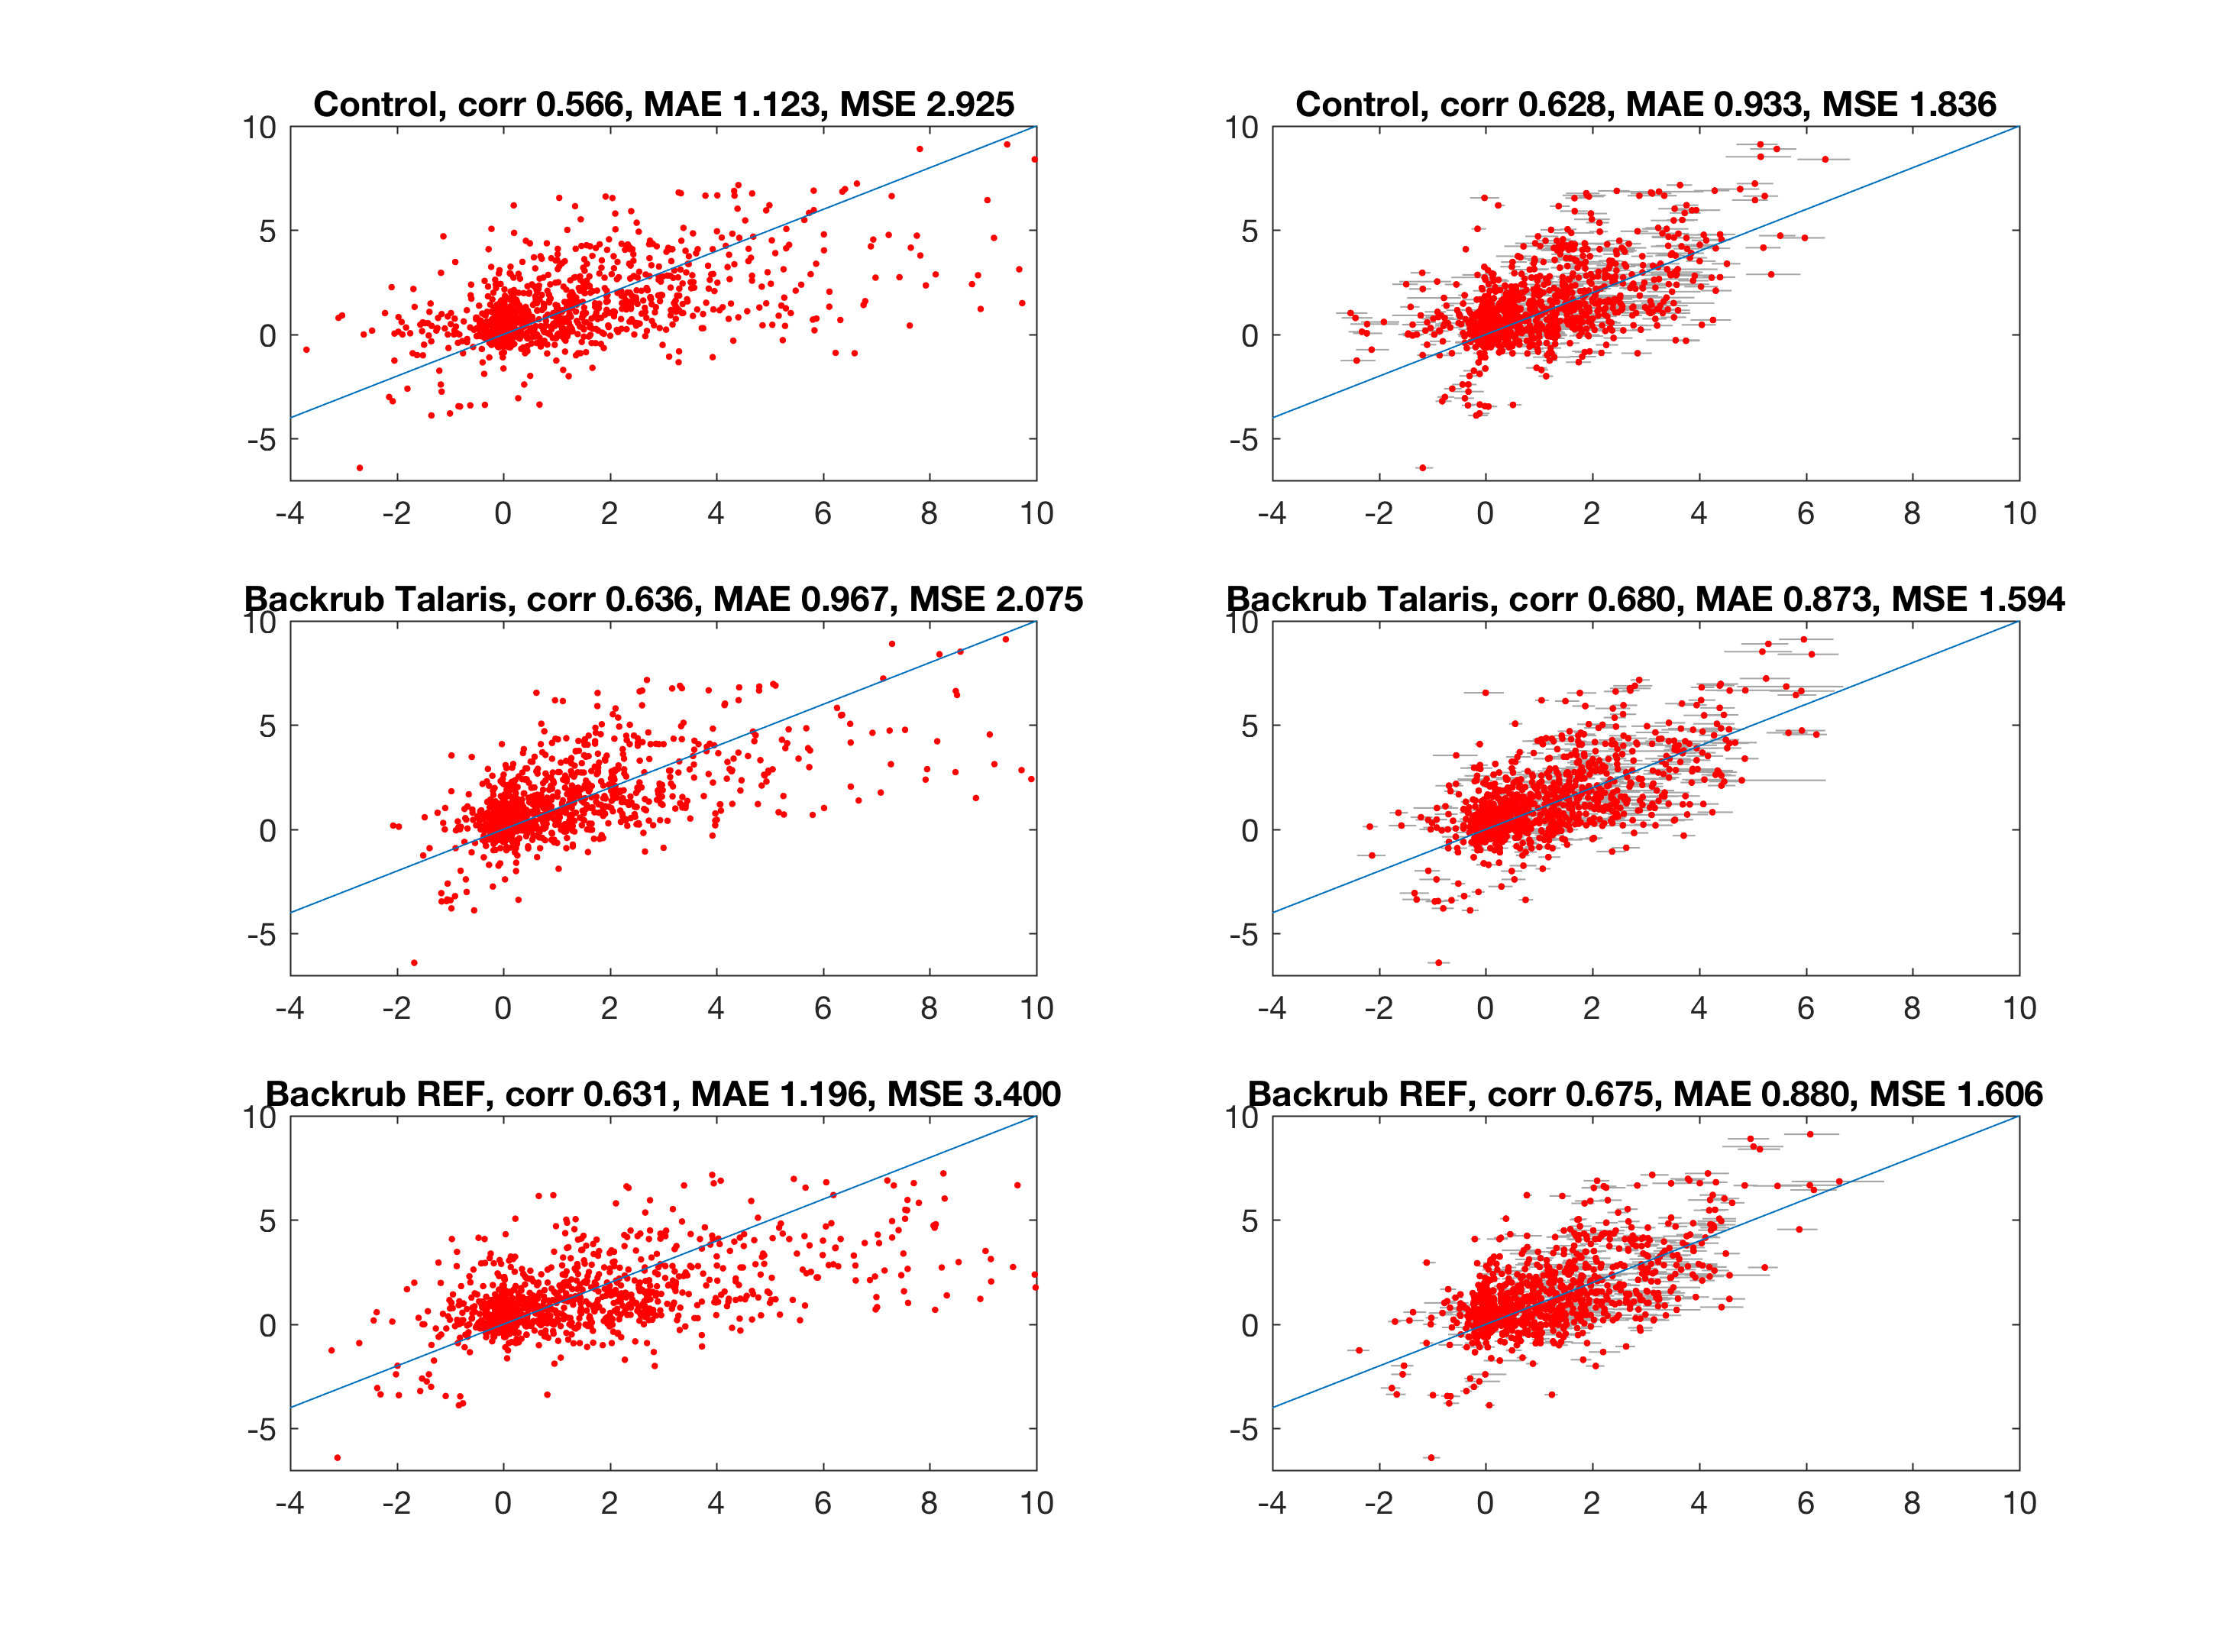
\includegraphics[width=\textwidth,keepaspectratio]{figures/zemu-sigmoid2-corrs.png}
%   \caption[Interface \ddg prediction performance with sigmoid fit score function]{
%     Left: standard flex ddG Rosetta output (non-fitted predictions) vs. experimental \ddg\ values. Right: Generalized additive model (GAM) flex ddG predictions vs. experimental data. Top: Control (no backrub) predictions. Middle: Flex ddG run with the Talaris energy function for 30,000 backrub steps with kT=1.2, averaged over 50 output scores. Bottom: Flex ddG run with the REF energy function, also for 30,000 backrub steps with kT=1.2, averaged over 50 output scores. The GAM is able to reduce the number of outlier flex ddG predictions, particularly relatively neutral values that Rosetta predicts to be highly destabilizing. This improvement in performance is most likely due to the ability of the sigmoid member functions of the GAM to limit extreme score term values once they are no longer predictive.
%   } \label{fig:t14-fit-scatter}
% \end{figure}

\begin{figure}
  \centering
  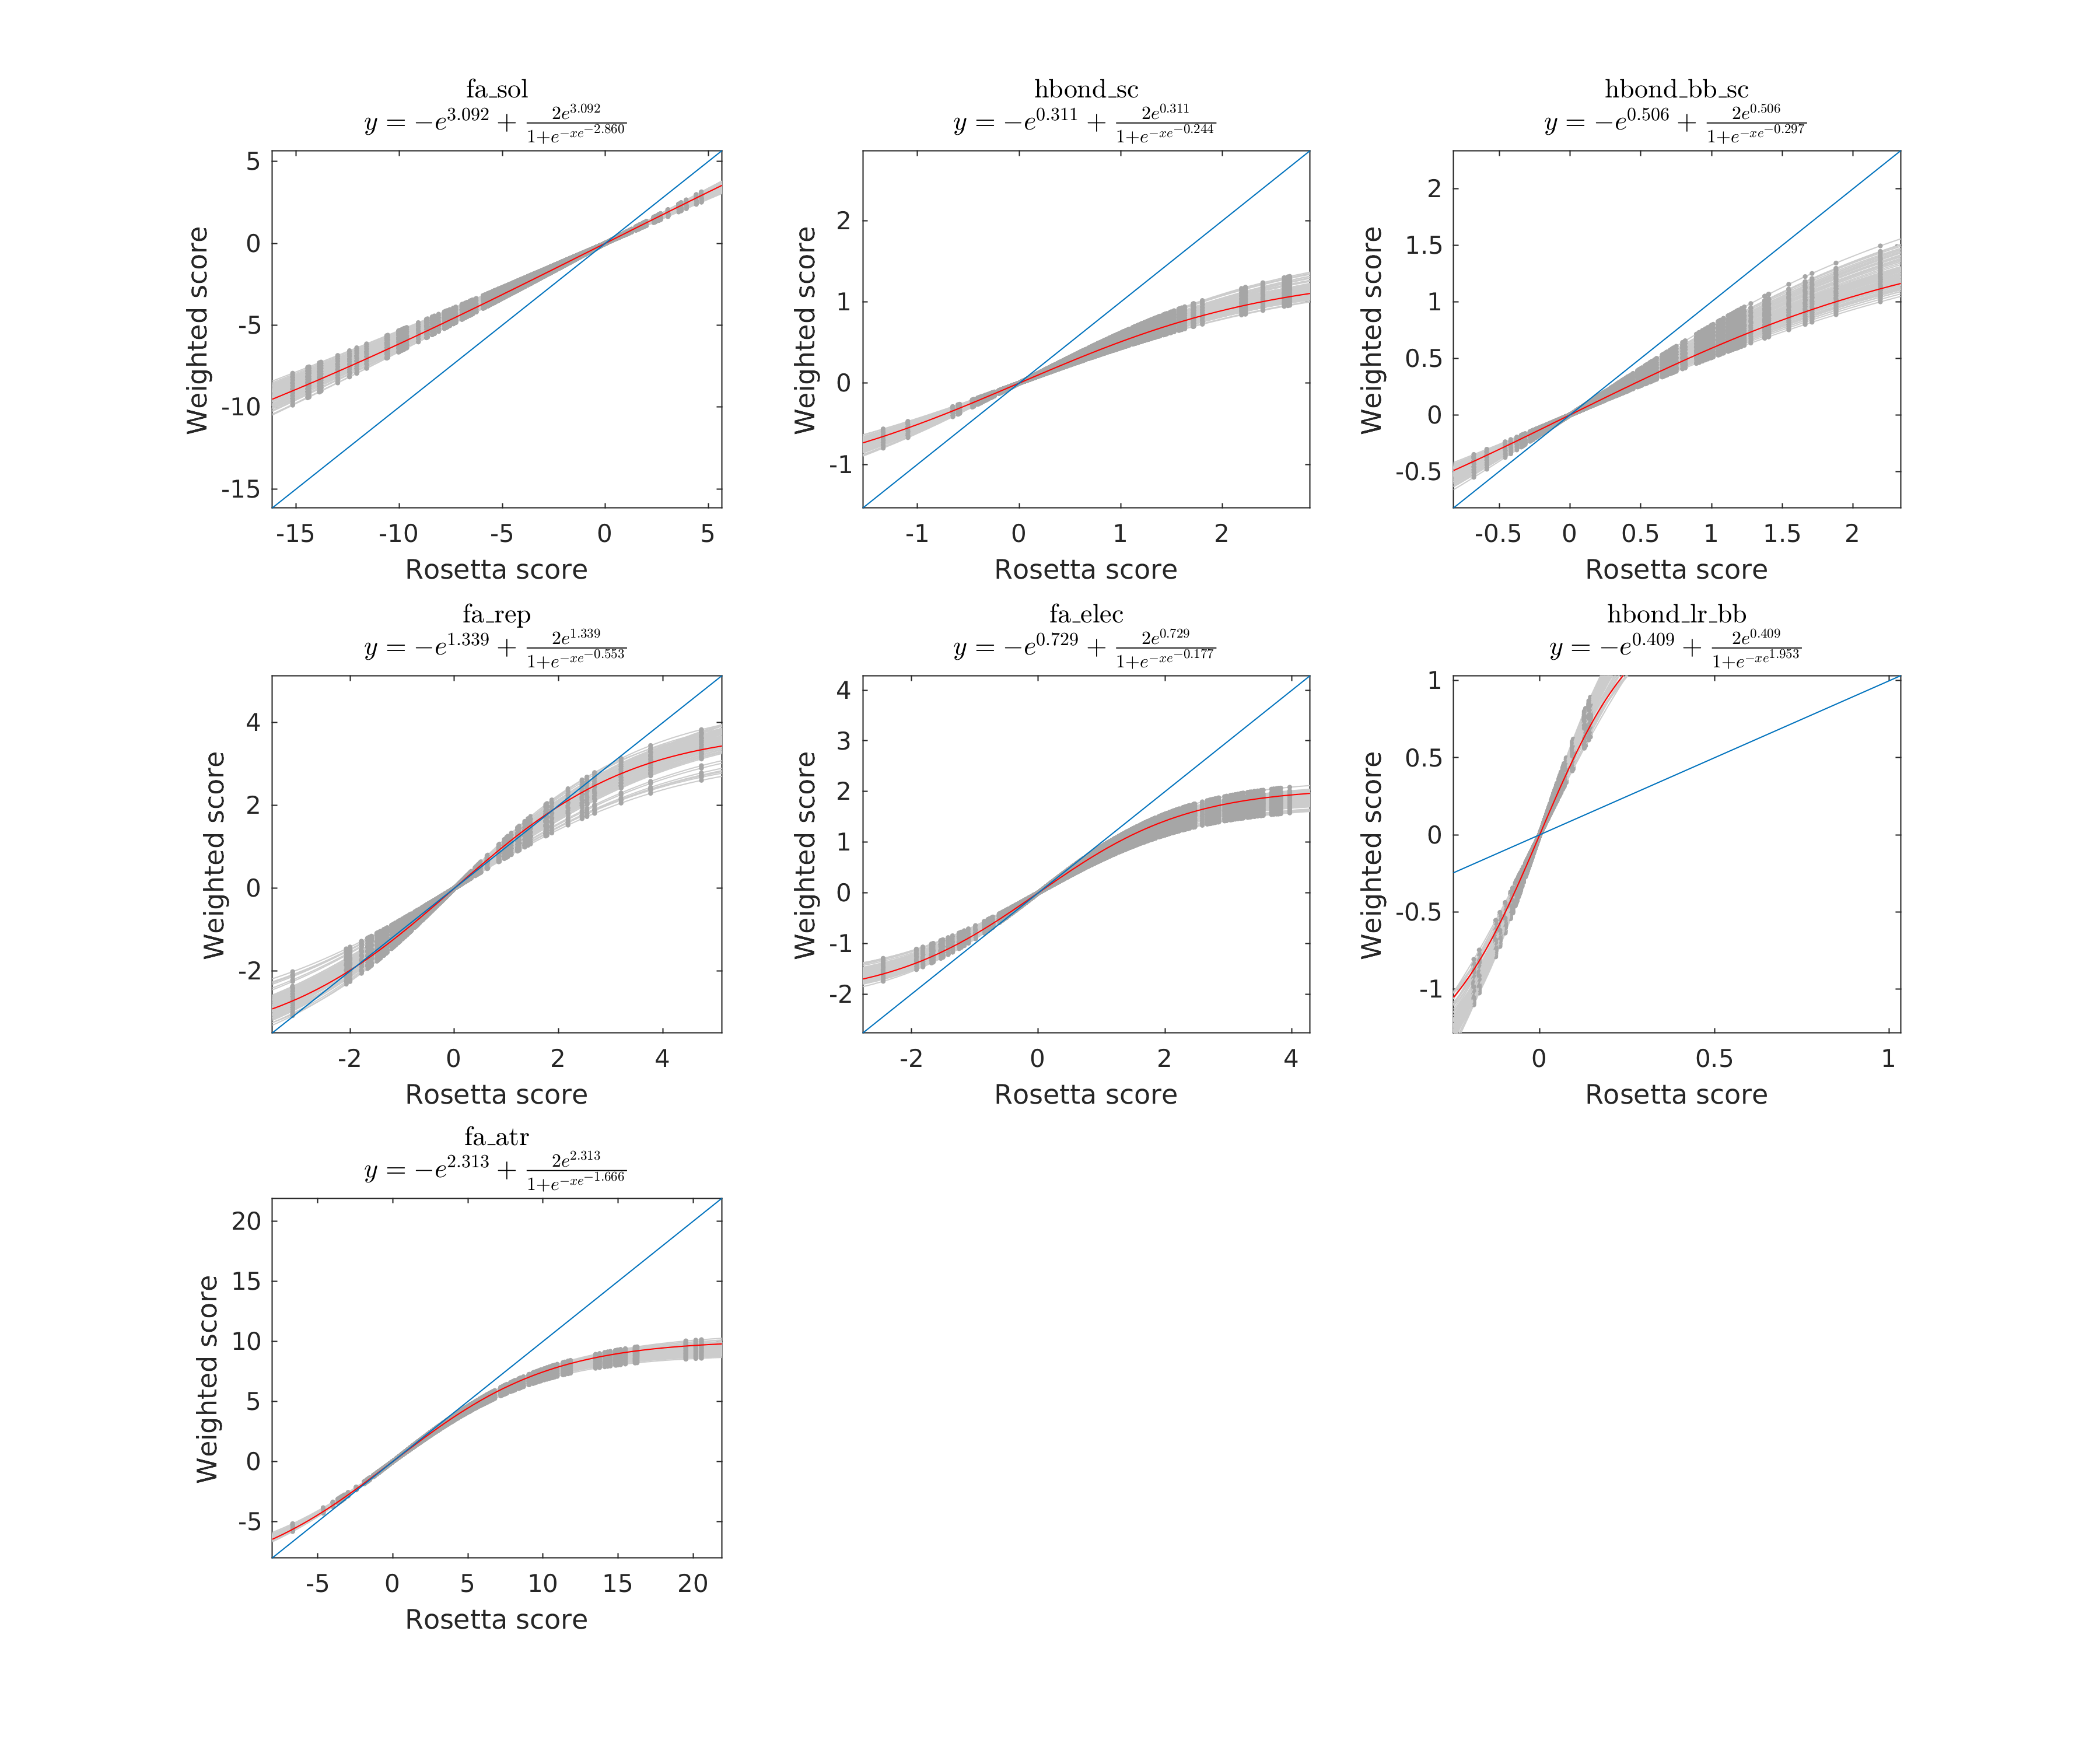
\includegraphics[width=\textwidth,keepaspectratio]{figures/zemu-sigmoid2-tal-feats.png}
  \caption[Sigmoid fit Rosetta score function terms]{
    Sigmoid functions resulting from application of unbiased logistic scaling to individual Rosetta score terms (generated using the flex ddG protocol and the Talaris energy function) in a generalized additive model. Extreme values for most score terms are downweighted, except for long-range hydrogen bond interactions between backbone atoms (hbond\_lr\_bb).
  } \label{fig:t14-fits-feats}
\end{figure}

\subimport*{figs-and-tables/}{table-ref}

\begin{figure}
  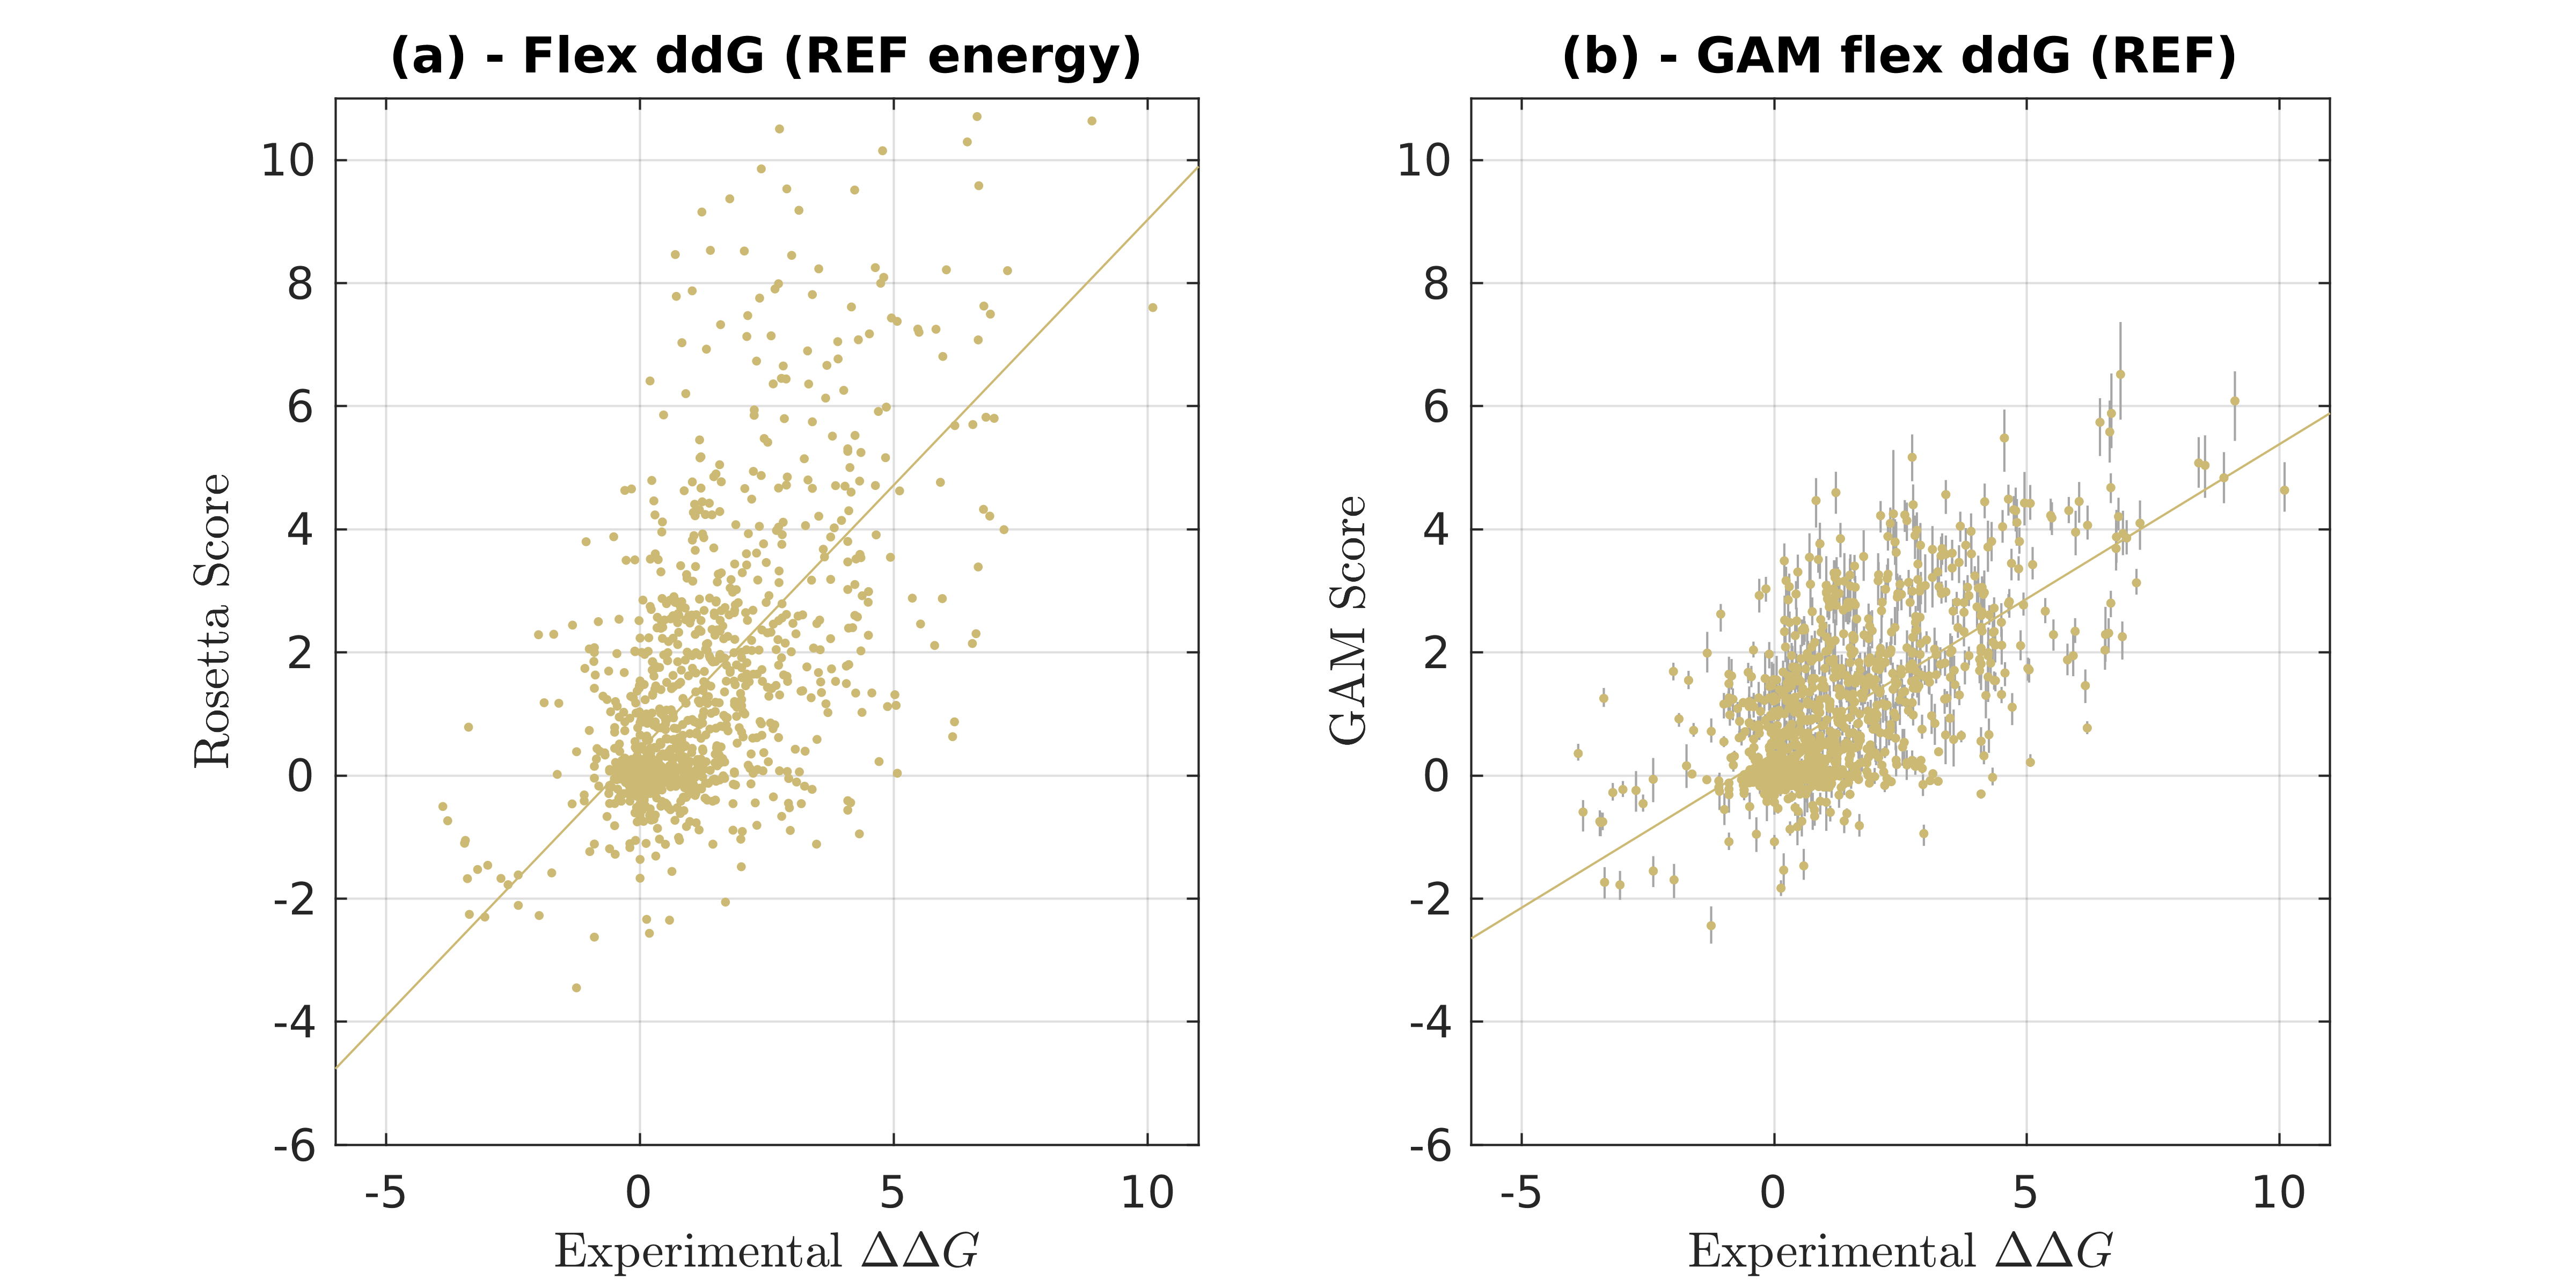
\includegraphics[width=\textwidth,keepaspectratio]{figures/zemu-sigmoid2-corrs-supp.png}
  \caption[]{
    \textbf{Left}: standard Rosetta output (non-fitted predictions) vs. experimental \ddg\ values.
    \textbf{Right}: Generalized additive model (GAM) flex ddG predictions vs. experimental data.
    The error bars in gray are represent the range from minimum to maximum fit predicted \ddg\ value for the 1000 sampled GAM models.
    Flex ddG Rosetta predictions were run with the REF energy function for 30,000 backrub steps with kT=1.2, averaged over 50 output scores.
    A line of of best fit is shown in each of the panels.
  } \label{fig:t14-fit-scatter-supp}
\end{figure}

\begin{table}
  \begin{tabular}{llrrrr}
\toprule
Prediction Method &     N &    R &  MAE &   FC \\
\midrule
 Flex ddG (talaris) GAM & \multirow{ 4}{*}{1240} & 0.68 & 0.87 & 0.76 \\
 Flex ddG (REF) GAM & & 0.68 & 0.88 & 0.75  \\
 No backrub control GAM & & 0.62 & 0.93 & 0.75  \\
\bottomrule
\end{tabular}
  \caption[]{
    Performance for GAM-fit predictions on the complete benchmark data set. Backrub steps = 35000. R = Pearson's R. MAE = Mean Absolute Error. FC = Fraction Correct. N = number of mutations in the dataset.
  } \label{tab:table-gam-fit}
\end{table}

\begin{figure}
  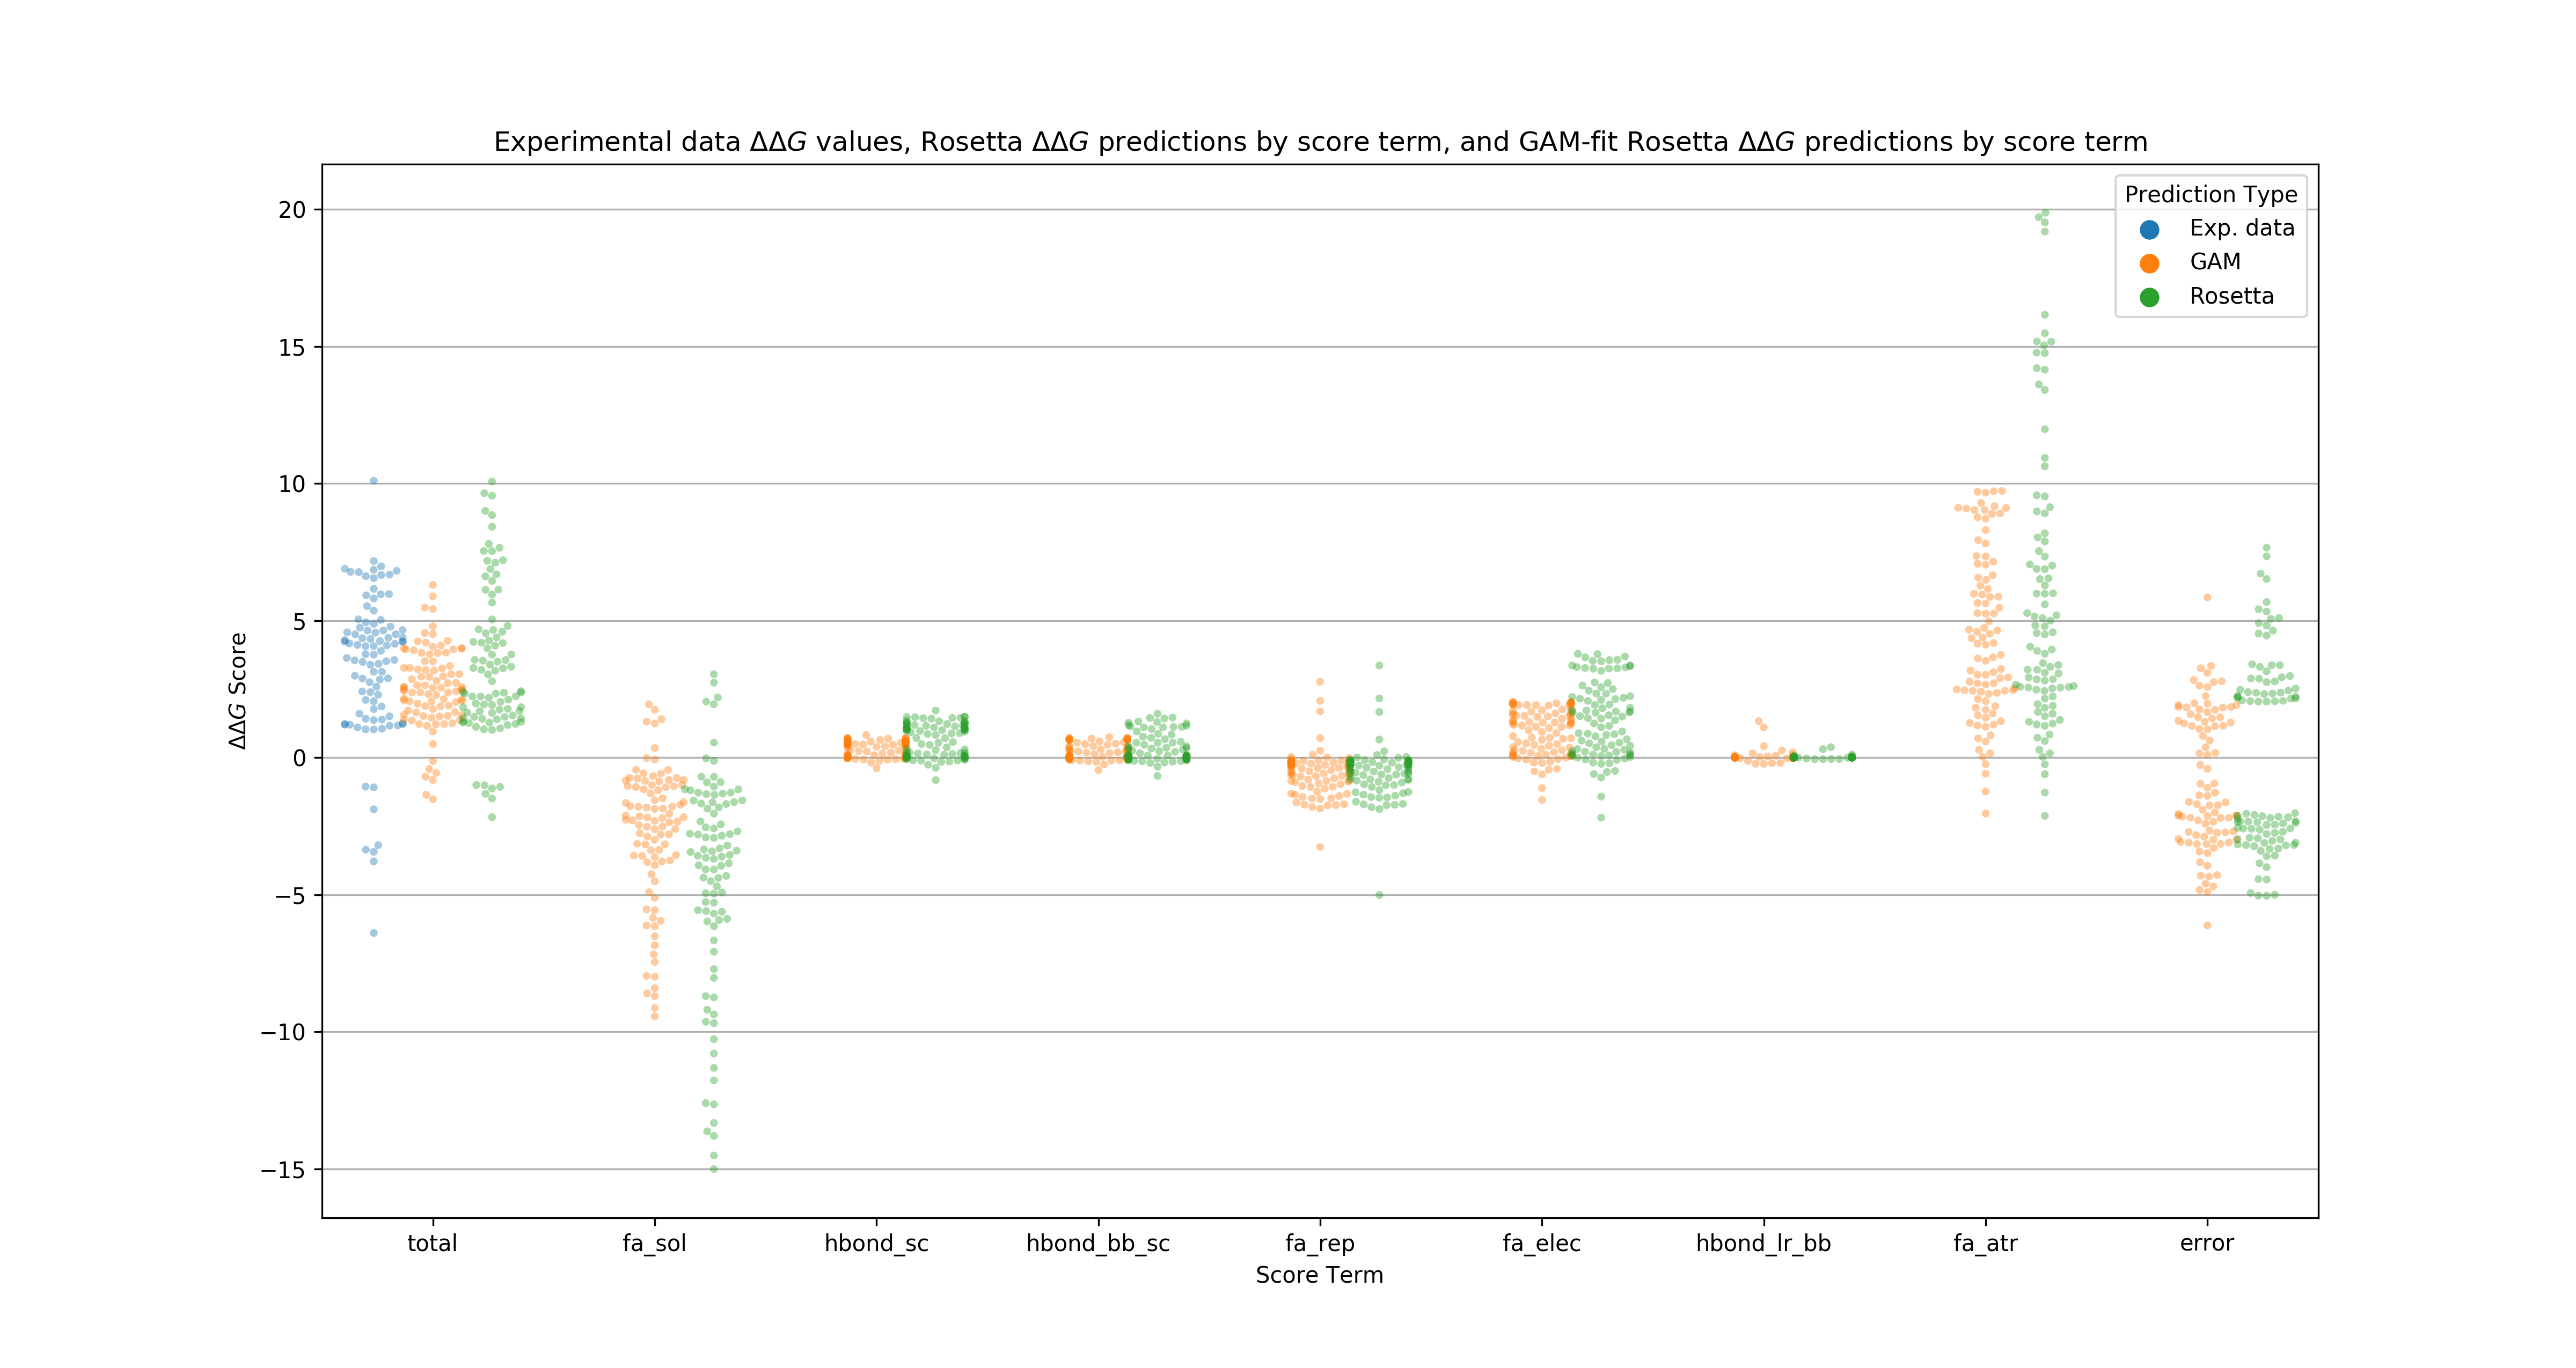
\includegraphics[width=\textwidth,keepaspectratio]{figures/tal_GAM_terms-mpl.png}
  \caption[]{
    Total \ddg\ predictions and partial Rosetta score terms (talaris energy function). On the far left, total scores for the original Rosetta predictions are shown in green alongside GAM-fit predictions in orange and the experimentally determined values in blue. On the far right, the error ($\Delta\Delta G_{predicted} - \Delta\Delta G_{experimental}$) is shown. Intermediate strips show the 7 partial Rosetta score terms (fa\_sol, hbond\_sc, hbond\_bb\_sc, hbond\_lr\_bb, fa\_rep, fa\_elec, and fa\_atr) which together equal the total \ddg\ score on the far left.
    Points shown are filtered from the complete prediction set according to the following criteria: neutral mutations are removed (-1.0 $<$ experimental \ddg\ or Rosetta predicted \ddg\ score $<$ 1.0). Also removed are points where the absolute value of the error of the original Rosetta prediction is less than 2.0
  } \label{fig:tal-GAM-terms-mpl}
\end{figure}

\clearpage

\renewcommand{\thetable}{Dataset \arabic{table}}
\setcounter{table}{0}

\csvreader[
longtable=|c|c|c|p{8cm}|r|,
table head=\caption{Curated ZEMu dataset with experimental \ddg\ values}\label{dst:zemu-filtered}\\\hline
ID & PDB & Res. & Mutations & \ddg\\\hline
\endhead\hline\endfoot,
% \csvlinetotablerow\\\hline
% \endfirsthead\hline
% \csvlinetotablerow\\\hline
% \endhead\hline
% \endfoot,
]
{figures/table-zemu-filtered.csv}
{1=\DataSetID,2=\PDBFileID,3=\Resolution,4=\Mutations,5=\ExperimentalDDG}
{\DataSetID & \PDBFileID & \Resolution & \Mutations & \ExperimentalDDG}

\captionof{listing}{
  Flex ddg Rosetta Script implementation
  \label{lst:ddg-script}
}
\inputminted[
linenos=true,
% frame=single,
breaklines
]
{xml}
{listings/ddG-backrub.xml}

\clearpage

\end{document}